%%%%%%%%%%%%%%%%%%%%%%%%%%%%%%%%%%%%%%%%%%%%%%%%%%%%%%%%%%%%%%%%%%%%%%%%%%%%
% AGUJournalTemplate.tex: this template file is for articles formatted with LaTeX
%
% This file includes commands and instructions
% given in the order necessary to produce a final output that will
% satisfy AGU requirements, including customized APA reference formatting.
%
% You may copy this file and give it your
% article name, and enter your text.
% guidelines and troubleshooting are here: 

%% To submit your paper:
%% NOTES:
% DON'T USE SUBFIGURES!!!!



\documentclass[draft]{AR_analysis_}
% \usepackage{hyperref} % creates a hyperlink to the figure referenced
\usepackage{url} %this package should fix any errors with URLs in refs.
\usepackage{lineno}
%for better track changes. finalnew option will compile document with changes incorporated.
\usepackage[inline]{trackchanges}
\usepackage{soul}
\usepackage{float}  % Required for the [H] option
\usepackage{graphicx} % for my graphics
\usepackage{xcolor} % for my graphics
\usepackage{textcomp} % removes warning in gensymb
\usepackage{gensymb} % for basic symbols like degree
\usepackage{mathtools}
\usepackage{amsmath}
\usepackage{tabularx}
%\usepackage{subcaption}

\usepackage{makecell}
\usepackage{array}

\newcolumntype{R}[1]{>{\raggedleft\arraybackslash}m{#1}}

% Bottom four packages from matplotlib -> LaTeX 
% Tutorial
% https://blog.timodenk.com/exporting-matplotlib-plots-to-latex/
\usepackage{tikz}
\usepackage{tikz-cd}
\usepackage{pgfplots}
\pgfplotsset{compat=1.14}

\linenumbers

%%%%%%%
% As of 2018 we recommend use of the TrackChanges package to mark revisions.
% The trackchanges package adds five new LaTeX commands:
%
%  \note[editor]{The note}
%  \annote[editor]{Text to annotate}{The note}
%  \add[editor]{Text to add}
%  \remove[editor]{Text to remove}
%  \change[editor]{Text to remove}{Text to add}
%
% complete documentation is here: http://trackchanges.sourceforge.net/
%%%%%%%

\draftfalse

%% Enter journal name below.
%% Choose from this list of Journals:
%
% JGR: Atmospheres
% JGR: Biogeosciences
% JGR: Earth Surface
% JGR: Oceans
% JGR: Planets
% JGR: Solid Earth
% JGR: Space Physics
% Global Biogeochemical Cycles
% Geophysical Research Letters
% Paleoceanography and Paleoclimatology
% Radio Science
% Reviews of Geophysics
% Tectonics
% Space Weather
% Water Resources Research
% Geochemistry, Geophysics, Geosystems
% Journal of Advances in Modeling Earth Systems (JAMES)
% Earth's Future
% Earth and Space Science
% Geohealth
%
% ie, \journalname{Water Resources Research}

\journalname{Geophysical Research Letters}

\begin{document}

%%%%%%%%%%%%%%%%%%%%%%%%%%%%%%%%%%%%%%%%%%%%%%%
%  TITLE
%
% (A title should be specific, informative, and brief. Use
% abbreviations only if they are defined in the abstract. Titles that
% start with general keywords then specific terms are optimized in
% searches)
%
%%%%%%%%%%%%%%%%%%%%%%%%%%%%%%%%%%%%%%%%%%%%%%%

\title{Influence of Atmospheric Rivers on Alaskan River Ice}

%%%%%%%%%%%%%%%%%%%%%%%%%%%%%%%%%%%%%%%%%%%%%%%
%
%  AUTHORS AND AFFILIATIONS
%
%%%%%%%%%%%%%%%%%%%%%%%%%%%%%%%%%%%%%%%%%%%%%%%

% Authors are individuals who have significantly contributed to the
% research and preparation of the article. Group authors are allowed, if
% each author in the group is separately identified in an appendix.)

% List authors by first name or initial followed by last name and
% separated by commas. Use \affil{} to number affiliations, and
% \thanks{} for author notes.
% Additional author notes should be indicated with \thanks{} (for
% example, for current addresses).

\authors{Russ Limber\affil{1, 2}, Elias Massoud\affil{2}, Jitendra Kumar\affil{2}, Forrest M. Hoffman\affil{2}}
\affiliation{1}{The University of Tennessee}
\affiliation{2}{Oak Ridge National Laboratory}

% \affiliation{3}{Third Affiliation}
% \affiliation{4}{Fourth Affiliation}

%(repeat as many times as is necessary)

% Corresponding author mailing address and e-mail address:

% (include name and email addresses of the corresponding author.  More
% than one corresponding author is allowed in this LaTeX file and for
% publication; but only one corresponding author is allowed in our
% editorial system.)

% Example: \correspondingauthor{First and Last Name}{email@address.edu}
\correspondingauthor{Russ Limber}{r62@ornl.gov}


%%%%%%%%%%%%%%%%%%%%%%%%%%%%%%%%%%%%%%%%%%%%%%%
% KEY POINTS
%%%%%%%%%%%%%%%%%%%%%%%%%%%%%%%%%%%%%%%%%%%%%%%
%  List up to three key points (at least one is required)
%  Key Points summarize the main points and conclusions of the article
%  Each must be 140 characters or fewer with no special characters 
% or punctuation and must be complete sentences

% Example:
% \begin{keypoints}
% \item	List up to three key points (at least one is required)
% \item	Key Points summarize the main points and conclusions of the article
% \item	Each must be 140 characters or fewer with no special characters or punctuation and must be complete sentences
% \end{keypoints}

% These are all under 140 characters
\begin{keypoints}
\item Atmospheric Rivers (ARs) correlate to a one week increase in daily minimum temperature

\item Robust ARs occuring during the coldest period of the year appear to prolong the annual breakup
date of river ice

\item ARs account for about one third (36\%) of total precipitation and explain almost half (48\%)
 of interannual variability of precipitation
\end{keypoints}

%%%%%%%%%%%%%%%%%%%%%%%%%%%%%%%%%%%%%%%%%%%%%%%
%
%  ABSTRACT and PLAIN LANGUAGE SUMMARY
%
% A good Abstract will begin with a short description of the problem
% being addressed, briefly describe the new data or analyses, then
% briefly states the main conclusion(s) and how they are supported and
% uncertainties.

% The Plain Language Summary should be written for a broad audience,
% including journalists and the science-interested public, that will not have 
% a background in your field.
%
% A Plain Language Summary is required in GRL, JGR: Planets, JGR: Biogeosciences,
% JGR: Oceans, G-Cubed, Reviews of Geophysics, and JAMES.
% see http://sharingscience.agu.org/creating-plain-language-summary/)
%
%%%%%%%%%%%%%%%%%%%%%%%%%%%%%%%%%%%%%%%%%%%%%%%

%% \begin{abstract} starts the second page
%% The Abstract should be a single paragraph of fewer than 250 words
%% (for Geophysical Research Letters, under 150 words). 

\begin{abstract}

	Atmospheric rivers (ARs) transport vast amounts of moisture from
	low latitudes, mainly the Tropics, to high latitude regions. 
	One region particularly impacted
	by ARs is Alaska USA. We analyze the role of ARs in raising local temperatures, 
	their effect on precipitation variability, and their influence on the annual river
	ice breakup date for 25 locations. Precipitation and 
	temperature records were provided by Daymet, with ARs determined from the Guan and 
	Waliser tracking algorithm. We found ARs increase local temperatures for as long as 
	one week post landfall, account for 36\% of total precipitation and explain 48\% 
	of precipitation variability. Calculating the heat transport between ARs and river 
	ice, fused with a temporal bias, we conclude that heavy precipitation events 
	(HPEs) during the coldest period of the year prolong river ice breakup dates, 
	while HPEs occurring close to the breakup date have little impact on breakup timing. 

\end{abstract}

% The PLS should be a single paragraph no more than 200 words long.
\section*{Plain language summary}

	We strategically selected 25 locations with annual river ice
	breakup dates recorded throughout Interior Alaska. Across all
	locations, we determined that daily temperature increases by up to
	one week post an atmospheric river (AR). We also found that ARs
	account for 36\% of total annual precipitation from 1980 to 2023
	and explain 48\% of the variability of precipitation. We then
	calculated the total heat transfer between precipitation and river
	ice while taking into account a bias function for time.
	Surprisingly, we found that heavy precipitation events (HPEs),
	both local precipitation and ARs, that occur relatively close to
	river ice breakup dates, have little correlation to the breakup
	date. However, HPEs that occur during the coldest period of the
	year (typically late December to mid-January) are strongly inversely
	correlated with river ice breakup timing, and therefore prolong
	the breakup date.

%%%%%%%%%%%%%%%%%%%%%%%%%%%%%%%%%%%%%%%%%%%%%%%
%
%  BODY TEXT
%
%%%%%%%%%%%%%%%%%%%%%%%%%%%%%%%%%%%%%%%%%%%%%%%

%%% Suggested section heads:
% \section{Introduction}
%
% The main text should start with an introduction. Except for short
% manuscripts (such as comments and replies), the text should be divided
% into sections, each with its own heading.

% Headings should be sentence fragments and do not begin with a
% lowercase letter or number. Examples of good headings are:

% \section{Materials and Methods}
% Here is text on Materials and Methods.
%
% \subsection{A descriptive heading about methods}
% More about Methods.
%
% \section{Data} (Or section title might be a descriptive heading about data)
%
% \section{Results} (Or section title might be a descriptive heading about the
% results)
%
% \section{Conclusions}



\section{Introduction}

Atmospheric rivers (ARs) are narrow corridors of intense water vapor transport that 
significantly influence hydrologic events and transport most of the 
water vapor outside of the Tropics \cite{NOAA_AR_summary}. It is estimated that ARs
are responsible for as much as 90\% of poleward water vapor transport at 
midlatitudes \cite{other_alg}. ARs contribute to extreme precipitation events across various 
regions worldwide, including western North America
\cite{Dettinger2004, Guan2010, ARs_flood_WA_State, 
ARs_flood_Russian_River_CA, Ralph2013, ARs_CA} 
Europe \cite{Lavers2013, ARs_impact_Norway}, and western South America 
\cite{ARs_impact_SA}. In recent years, the impacts of ARs on the cryosphere have been more
extensively anlayzed. It was found that
between 1981 and 2020 atmospheric moisture content anticorrelates
significantly with sea ice concentration over almost the entire Arctic
Ocean \cite{ARs_lead_to_sea_ice_loss}. For those same years, another
analysis found that 100\% of extreme temperature events in the Arctic (above 0
$\degree C$) coincided with ARs \cite{Ma2023}. Many analyses have
noted a relationship between heavy AR activity and sea ice loss, as a
result of increased rainfall from lower latitudues 
\cite{Zhang2023, maclennan_contribution_2022}.
However Arctic systems are complicated, as the intense moisture 
transport within ARs can also result in heavy snowfall events, thus contributing to 
the accumulation of snowpack, especially in mountainous regions 
\cite{Saavedra2020, Guan2010}. Under the right conditions, this
relationship has been found to increase the mass balance of glaciers
\cite{Little2019}. Understanding the role of ARs in the cryosphere is 
essential for assessing their broader impact 
on regional water resources and glacier dynamics in a changing climate.
While a number of works have explored the relationship
between ARs and sea ice, to our knowledge there haven't been any
analyses that look at the relationship between ARs and Arctic river ice.
Many works have used physics based processes and allometrics to model 
the annual breakup timing and conditions of Arctic river ice 
\cite{Paily, ashton1986river, Prowse_Bonsal_Duguay_Lacroix_2007, jasek1998, shen_newest}.
While it is recognized that an increase streamflow 
alters the dynamics surrounding river ice breakup timing
\cite{ashton1986river}, the relationship precipitation and to that end
AR timing has on Arctic river ice has yet to be examined. 
This analysis sets out to answer the following questions: 
1.) Is there a change in air
temperature for each location, corresponding to the timing of ARs? 
2.) How do ARs contribute to precipitation throughout interior Alaska?
3.) Do ARs impact the timing of river ice breakup?

\section{Data}

\begin{figure}
\centering
\includegraphics[width=1.0\textwidth]{./images/concatenated_maps_precip_temp_plot.png}
	\caption{Top: (left) map showing summated precipitation for the
	year 2021; (right) map of average temperature for 2021. Bottom:
	One of the 25 locations (Crooked Creek on the Kuskokwim
	River) for the year 2021. Yellow, orange, red represents the
	temperature profiles (fill plot of tmin - tmax) from NCEP
	temperature data at 850, 925 and 1000mb respectively. Light
	green represents Daymet temperature profile. Dark blue shows
	modeled precipitation from Daymet while the light blue stem
	plots depict AR events. The purple dashed line shows the breakup
	date for the Kuskokwim River in 2021 for Crooked Creek.}
\label{fig:concatenated_maps_precip_temp_plot} 
\end{figure}

\section{Methods}


\section{Results} 

\begin{figure}
\centering
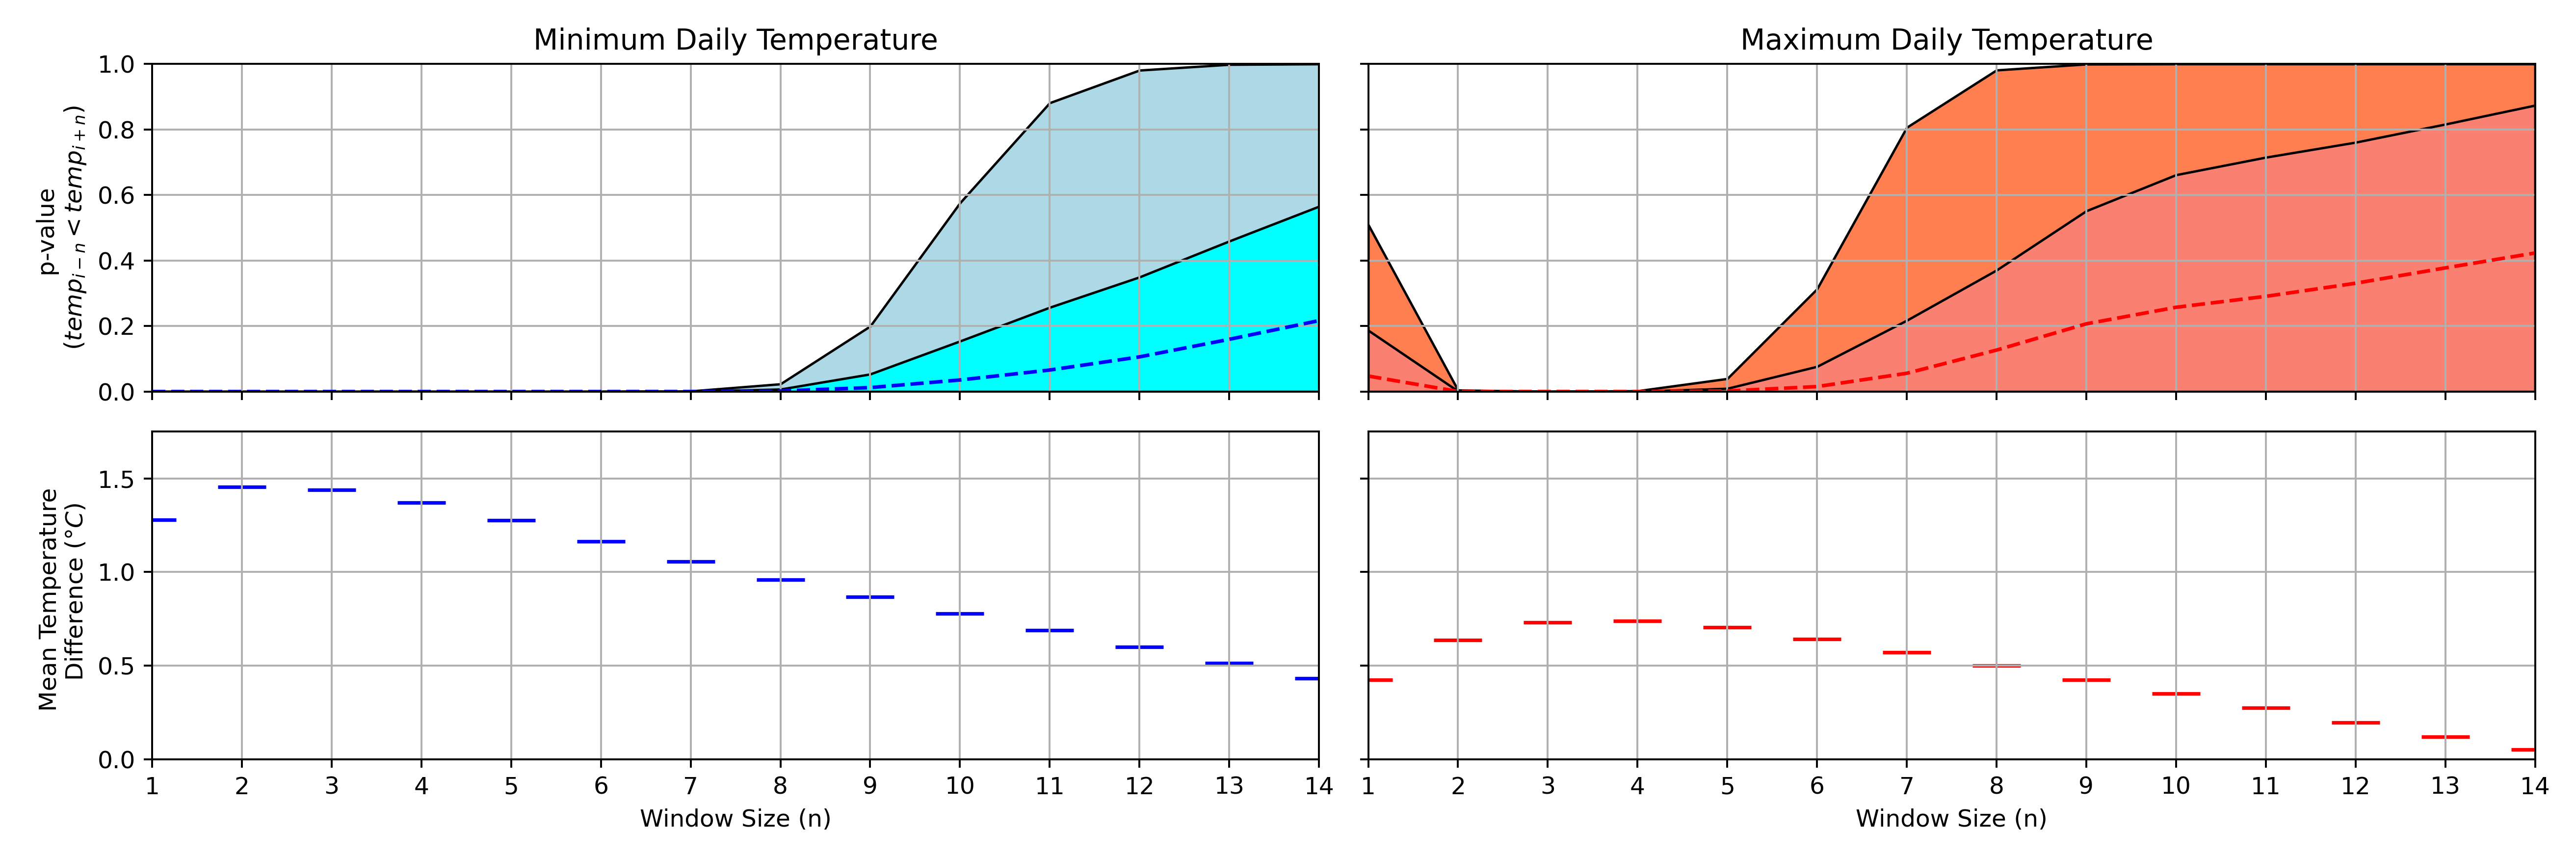
\includegraphics[width=1.0\textwidth]{./images/tmin_vs_tmax_subplots.png}
\caption{Top: the p-value of the paired t-test given the
	window size surrounding the AR event date. Dashed lines
	represent the mean p-value over the study area while the color
	transition depicts the IQR of p-values Bottom: the average increase
	in temperature from the lookback window to the forecast window.}
\label{fig:tmin_vs_tmax_subplots} 
\end{figure}

\begin{figure}
\centering
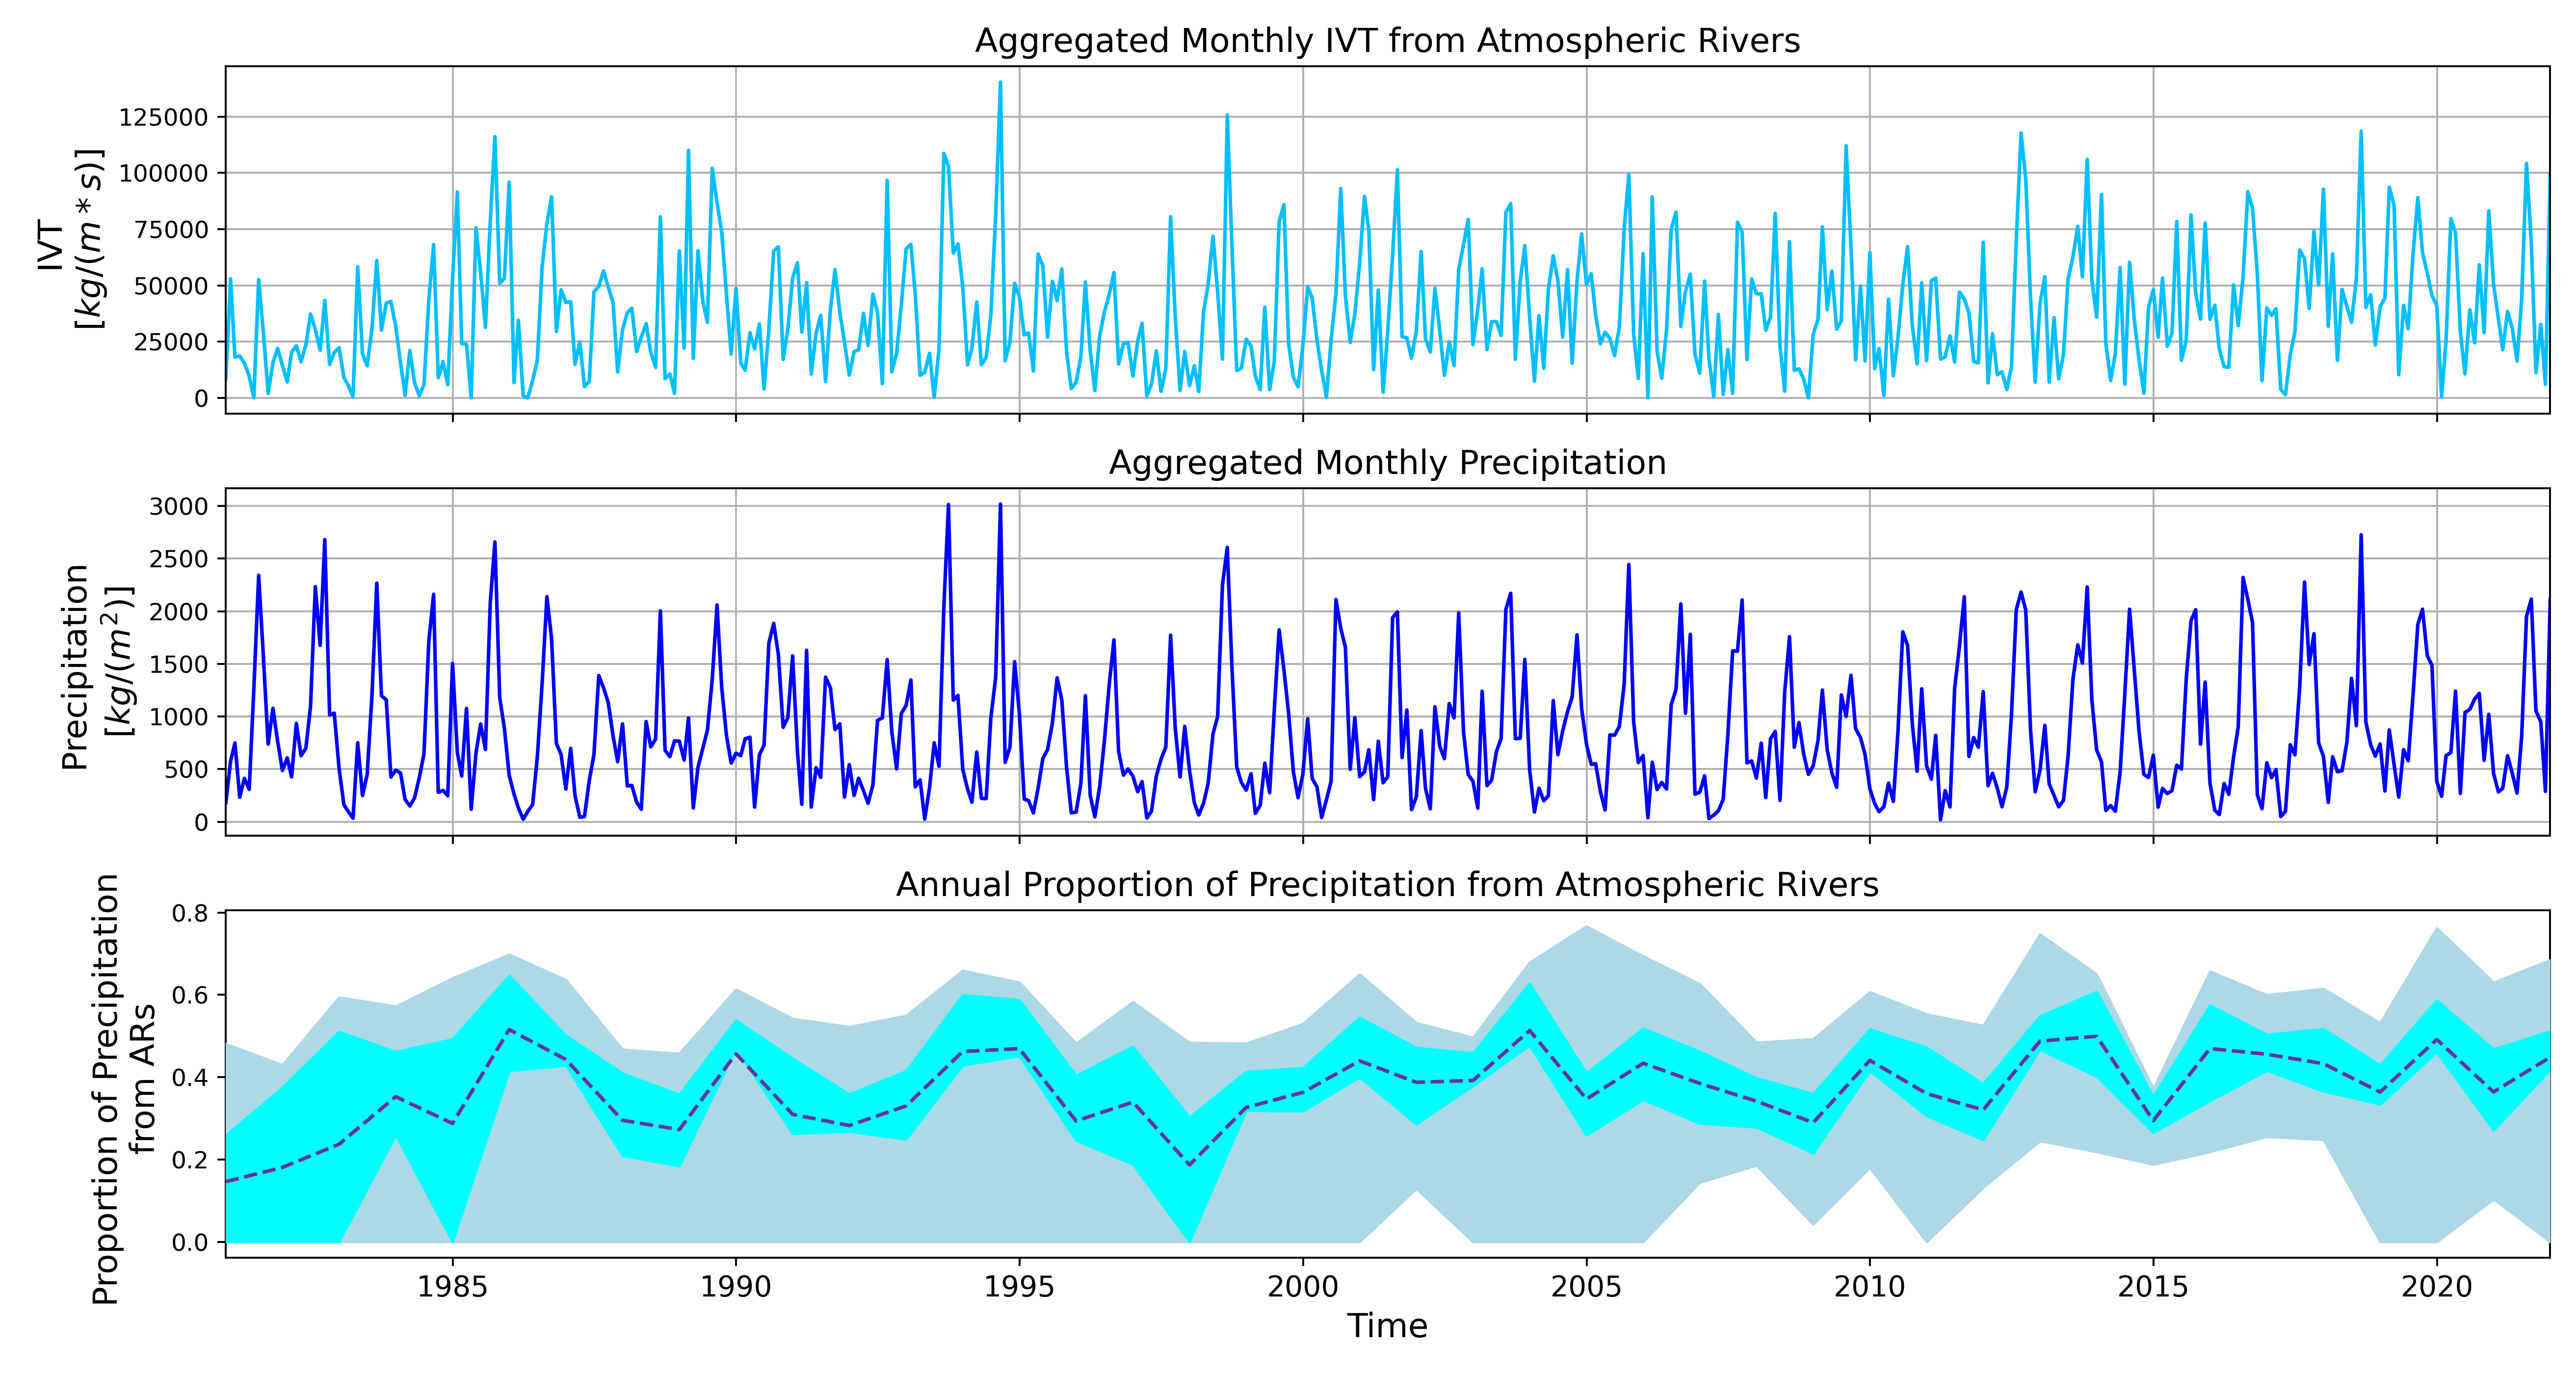
\includegraphics[width=1.0\textwidth]{./images/IVT_Precip_proportion_over_time.png}
\caption{Top: time series of IVT aggregated over all locations.
	Middle: time series of precipitation aggregated monthly over all
	locations. Bottom: proportion of precipitation accounted for by
	ARs, fill colors depict IQR while dashed line depicts the mean,
	aggregated over all locations annually. }
\label{fig:IVT_Precip_proportion_over_time}
\end{figure}

\begin{figure}
\centering
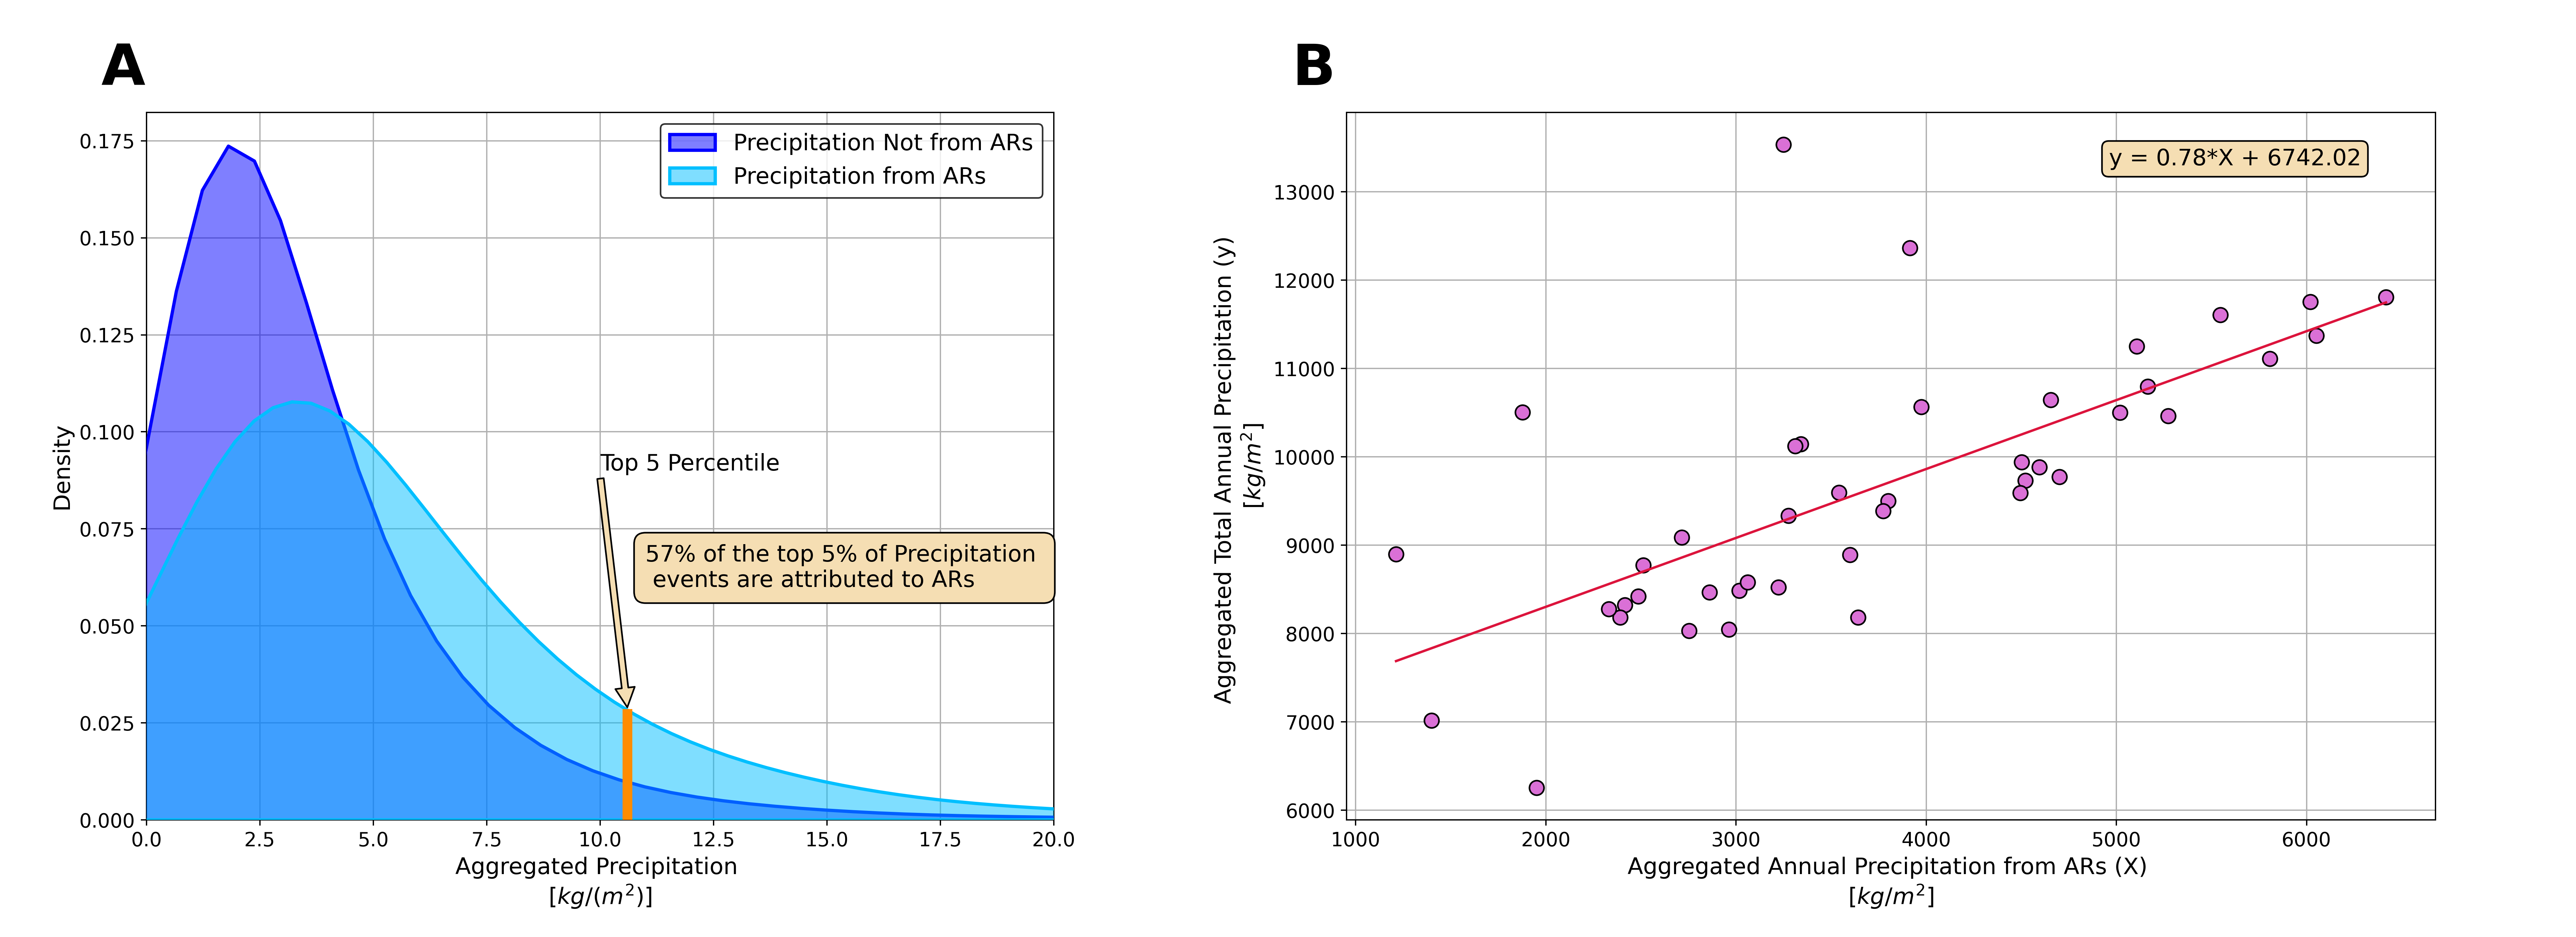
\includegraphics[width=1.0\textwidth]{./images/concatenated_precip_var_plots.png}
\caption{Left: kernel density plots showing the distribution of
	local precipitation (dark blue) and precipitation from ARs
	(light blue). Right: orindary least squares regression plot
	using annual, summated precipitation from ARs, to predict annual
	summated precipitation.}
\label{fig:concatenated_precip_var_plots}
\end{figure}

\begin{figure}
\centering
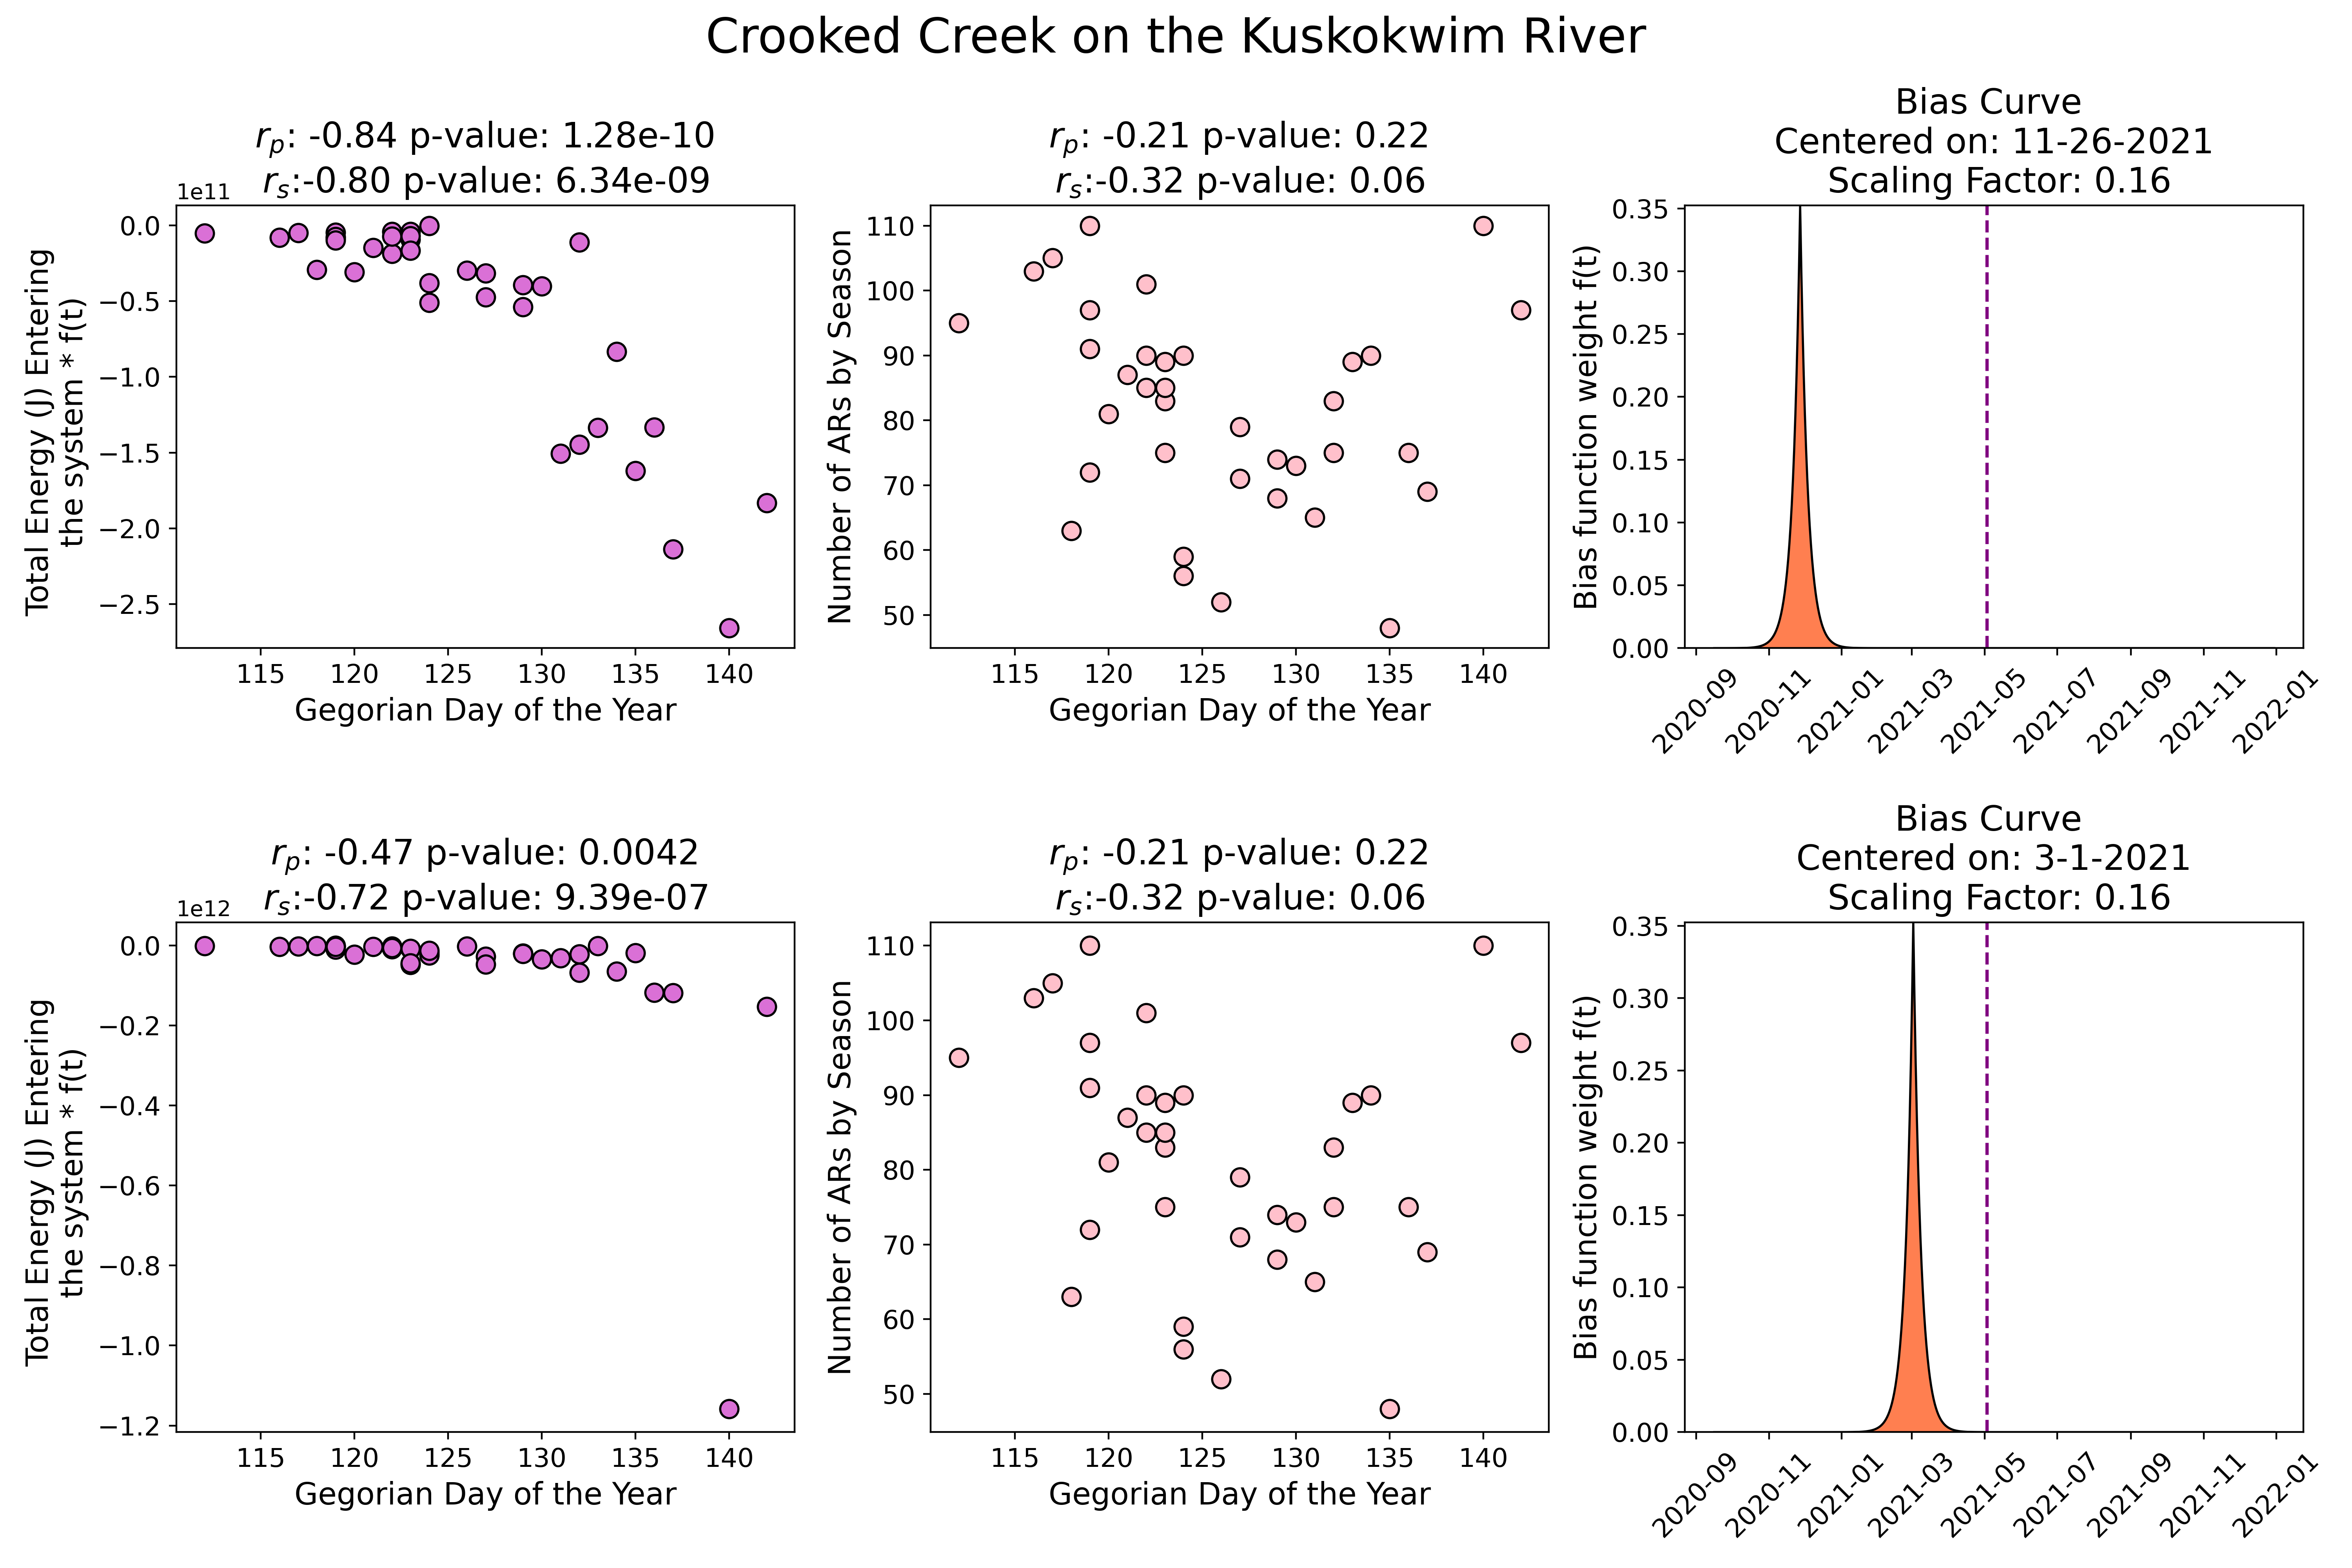
\includegraphics[width=1.0\textwidth]{./images/concatenated_corr_plots.png}
	\caption{Top: (left) scatter plot between thermal energy
	transfer and DOY; (middle) scatter plot of the number of ARs
	that occured in the 6 months prior to the breakup date and DOY 
	(right) temporal bias curve for the year 2021 with the breakup
	date represented by the vertical dashed ilne. Bottom: same as
	the top except depicting when the bias curve is not optimally
	placed (close to the breakup date).}
\label{fig:concatenated_corr_plots}
\end{figure}

\section{Conclusion}


%%%%%%%%%%%%%%%%%%%%%%%%%%%%%%%%%%%%%%%%%%%%%%%
%
% DATA SECTION and ACKNOWLEDGMENTS
%
%%%%%%%%%%%%%%%%%%%%%%%%%%%%%%%%%%%%%%%%%%%%%%%

\section*{Open research section}
This section MUST contain a statement that describes where the data supporting the conclusions
can be obtained. Data cannot be listed as ''Available from authors'' or stored solely in 
supporting information. Citations to archived data should be included in your reference
list. Wiley will publish it as a separate section on the paper’s page. Examples and 
complete information are here:
https://www.agu.org/Publish with AGU/Publish/Author Resources/Data for Authors


\acknowledgments
Enter acknowledgments here. This section is to acknowledge funding, thank colleagues, 
enter any secondary affiliations, and so on.


%%%%%%%%%%%%%%%%%%%%%%%%%%%%%%%%%%%%%%%%%%%%%%%
% REFERENCES and BIBLIOGRAPHY
%
% \bibliography{<name of your .bib file>} don't specify the file extension
% don't specify bibliographystyle
%
%%%%%%%%%%%%%%%%%%%%%%%%%%%%%%%%%%%%%%%%%%%%%%%

%\bibliography{ enter your bibtex bibliography filename here }
\bibliography{AR_analysis_}


%Reference citation instructions and examples:
%
% Please use ONLY \cite and \citeA for reference citations.
% \cite for parenthetical references
% ...as shown in recent studies (Simpson et al., 2019)
% \citeA for in-text citations
% ...Simpson et al. (2019) have shown...
%
%
%...as shown by \citeA{jskilby}.
%...as shown by \citeA{lewin76}, \citeA{carson86}, \citeA{bartoldy02}, and \citeA{rinaldi03}.
%...has been shown \cite{jskilbye}.
%...has been shown \cite{lewin76,carson86,bartoldy02,rinaldi03}.
%... \cite <i.e.>[]{lewin76,carson86,bartoldy02,rinaldi03}.
%...has been shown by \cite <e.g.,>[and others]{lewin76}.
%
% apacite uses < > for prenotes and [ ] for postnotes
% DO NOT use other cite commands (e.g., \citet, \citep, \citeyear, \nocite, \citealp, etc.).
%

\appendix
\section*{Appendix A.}


\end{document}






































% More Information and Advice:

%%

%  Numbered lines in equations:
%  To add line numbers to lines in equations,
%  \begin{linenomath*}
%  \begin{equation}
%  \end{equation}
%  \end{linenomath*}



%% Enter Figures and Tables near as possible to where they are first mentioned:
%
% DO NOT USE \psfrag or \subfigure commands.
%
% Figure captions go below the figure.
% Acronyms used in figure captions will be spelled out in the final, published version.

% Table titles go above tables;  other caption information
%  should be placed in last line of the table, using
% \multicolumn2l{$^a$ This is a table note.}
% NOTE that there is no difference between table caption and table heading in the final, published version
%
%----------------
% EXAMPLE FIGURES
%
% \begin{figure}
% \includegraphics{example.png}
% \caption{caption}
% \end{figure}
%
% Giving latex a width will help it to scale the figure properly. A simple trick is to use 
% \textwidth. Try this if large figures run off the side of the page.
% \begin{figure}
% \noindent\includegraphics[width=\textwidth]{anothersample.png}
%\caption{caption}
%\label{pngfiguresample}
%\end{figure}
%
%
% If you get an error about an unknown bounding box, try specifying the width and height 
% of the figure with the natwidth and natheight options. This is common when trying to add a PDF figure without pdflatex.
% \begin{figure}
% \noindent\includegraphics[natwidth=800px,natheight=600px]{samplefigure.pdf}
%\caption{caption}
%\label{pdffiguresample}
%\end{figure}
%
%
% PDFLatex does not seem to be able to process EPS figures. You may want to try the epstopdf package.
%

%
% ---------------
% EXAMPLE TABLE
%
% \begin{table}
% \caption{Time of the Transition Between Phase 1 and Phase 2$^{a}$}
% \centering
% \begin{tabular}{l c}
% \hline
%  Run  & Time (min)  \\
% \hline
%   $l1$  & 260   \\
%   $l2$  & 300   \\
%   $l3$  & 340   \\
%   $h1$  & 270   \\
%   $h2$  & 250   \\
%   $h3$  & 380   \\
%   $r1$  & 370   \\
%   $r2$  & 390   \\
% \hline
% \multicolumn{2}{l}{$^{a}$Footnote text here.}
% \end{tabular}
% \end{table}

%%%%%%%%%%%%%%%%%%%%%%%%%%%%%%%%%%%%%%%%%%%%%%%
% SIDEWAYS FIGURES and TABLES
% AGU prefers the use of {sidewaystable} over {landscapetable} as it causes fewer problems.
%
% \begin{sidewaysfigure}
% \includegraphics[width=20pc]{figsamp}
% \caption{caption here}
% \label{newfig}
% \end{sidewaysfigure}
%
%  \begin{sidewaystable}
%  \caption{Caption here}
% \label{tab:signif_gap_clos}
%  \begin{tabular}{ccc}
% one&two&three\\
% four&five&six
%  \end{tabular}
%  \end{sidewaystable}

%% If using numbered lines, please surround equations with \begin{linenomath*}...\end{linenomath*}
%\begin{linenomath*}
%\begin{equation}
%y|{f} \sim g(m, \sigma),
%\end{equation}
%\end{linenomath*}

%%% End of body of article

%%%%%%%%%%%%%%%%%%%%%%%%%%%%%%%%%%%%%%%%%%%%%%%
%% Optional Appendices go here
%
% The \appendix command resets counters and redefines section heads
%
% After typing \appendix
%
%\section{Here Is Appendix Title}
% will show
% A: Here Is Appendix Title
%

%%%%%%%%%%%%%%%%%%%%%%%%%%%%%%%%%%%%%%%%%%%%%%%
% Optional Glossary, Notation or Acronym section goes here:
%
% Glossary is only allowed in Reviews of Geophysics
%  \begin{glossary}
%  \term{Term}
%   Term Definition here
%  \term{Term}
%   Term Definition here
%  \term{Term}
%   Term Definition here
%  \end{glossary}


%%%%%%%%%%%%%%%%%%%%%%%%%%%%%%%%%%%%%%%%%%%%%%%
% Acronyms
%% NOTE that acronyms in the final published version will be spelled out when used in figure captions.
%   \begin{acronyms}
%   \acro{Acronym}
%   Definition here
%   \acro{EMOS}
%   Ensemble model output statistics
%   \acro{ECMWF}
%   Centre for Medium-Range Weather Forecasts
%   \end{acronyms}


%%%%%%%%%%%%%%%%%%%%%%%%%%%%%%%%%%%%%%%%%%%%%%%
% Notation
%   \begin{notation}
%   \notation{$a+b$} Notation Definition here
%   \notation{$e=mc^2$}
%   Equation in German-born physicist Albert Einstein's theory of special
%  relativity that showed that the increased relativistic mass ($m$) of a
%  body comes from the energy of motion of the body—that is, its kinetic
%  energy ($E$)—divided by the speed of light squared ($c^2$).
%   \end{notation}


%%%%%%%%%%%%%%%%%%%%%%%%%%%%%%%%%%%%%%%%%%%%%%%
%
%  SECTION HEADS
%
%%%%%%%%%%%%%%%%%%%%%%%%%%%%%%%%%%%%%%%%%%%%%%%

% Capitalize the first letter of each word (except for
% prepositions, conjunctions, and articles that are
% three or fewer letters).

% AGU follows standard outline style; therefore, there cannot be a section 1 without
% a section 2, or a section 2.3.1 without a section 2.3.2.
% Please make sure your section numbers are balanced.
% ---------------
% Level 1 head
%
% Use the \section{} command to identify level 1 heads;
% type the appropriate head wording between the curly
% brackets, as shown below.
%
%An example:
%\section{Level 1 Head: Introduction}
%
% ---------------
% Level 2 head
%
% Use the \subsection{} command to identify level 2 heads.
%An example:
%\subsection{Level 2 Head}
%
% ---------------
% Level 3 head
%
% Use the \subsubsection{} command to identify level 3 heads
%An example:
%\subsubsection{Level 3 Head}
%
%---------------
% Level 4 head
%
% Use the \subsubsubsection{} command to identify level 3 heads
% An example:
%\subsubsubsection{Level 4 Head} An example.
%
%%%%%%%%%%%%%%%%%%%%%%%%%%%%%%%%%%%%%%%%%%%%%%%
%
%  IN-TEXT LISTS
%
%%%%%%%%%%%%%%%%%%%%%%%%%%%%%%%%%%%%%%%%%%%%%%%
%
% Do not use bulleted lists; enumerated lists are okay.
% \begin{enumerate}
% \item
% \item
% \item
% \end{enumerate}
%
%%%%%%%%%%%%%%%%%%%%%%%%%%%%%%%%%%%%%%%%%%%%%%%
%
%  EQUATIONS
%
%%%%%%%%%%%%%%%%%%%%%%%%%%%%%%%%%%%%%%%%%%%%%%%

% Single-line equations are centered.
% Equation arrays will appear left-aligned.

%Math coded inside display math mode \[ ...\]
% will not be numbered, e.g.,:
% \[ x^2=y^2 + z^2\]

% Math coded inside \begin{equation} and %\end{equation} will
% be automatically numbered, e.g.,:
% \begin{equation}
% x^2=y^2 + z^2
% \end{equation}


% To create multiline equations, use the
% \begin{eqnarray} and \end{eqnarray} environment
% as demonstrated below.
%\begin{eqnarray}
 % x_{1} & = & (x - x_{0}) \cos \Theta \nonumber \\
 %       && + (y - y_{0}) \sin \Theta  \nonumber \\
%  y_{1} & = & -(x - x_{0}) \sin \Theta \nonumber \\
 %       && + (y - y_{0}) \cos \Theta.
%\end{eqnarray}

%If you don't want an equation number, use the star form:
%\begin{eqnarray*}...\end{eqnarray*}

% Break each line at a sign of operation
% (+, -, etc.) if possible, with the sign of operation
% on the new line.

% Indent second and subsequent lines to align with
% the first character following the equal sign on the
% first line.

% Use an \hspace{} command to insert horizontal space
% into your equation if necessary. Place an appropriate
% unit of measure between the curly braces, e.g.
% \hspace{1in}; you may have to experiment to achieve
% the correct amount of space.


%%%%%%%%%%%%%%%%%%%%%%%%%%%%%%%%%%%%%%%%%%%%%%%
%
%  EQUATION NUMBERING: COUNTER
%
%%%%%%%%%%%%%%%%%%%%%%%%%%%%%%%%%%%%%%%%%%%%%%%

% You may change equation numbering by resetting
% the equation counter or by explicitly numbering
% an equation.

% To explicitly number an equation, type \eqnum{}
% (with the desired number between the brackets)
% after the \begin{equation} or \begin{eqnarray}
% command.  The \eqnum{} command will affect only
% the equation it appears with; LaTeX will number
% any equations appearing later in the manuscript
% according to the equation counter.
%

% If you have a multiline equation that needs only
% one equation number, use a \nonumber command in
% front of the double backslashes (\\) as shown in
% the multiline equation above.

% If you are using line numbers, remember to surround
% equations with \begin{linenomath*}...\end{linenomath*}

%  To add line numbers to lines in equations:
%  \begin{linenomath*}
%  \begin{equation}
%  \end{equation}
%  \end{linenomath*}



